
\section{ ANTIGO }

Com a intenção cumprir com os objetivos descritos na seção \ref{cap:proposta}, o presente trabalho propõe a criação de uma aplicação web onde o usuário poderá configurar uma conta de \textit{WhatsApp} e realizar a coleta de mensagens de grupos públicos. Essa aplicação poderá se hospedada pelo usuário em sua própria máquina ou em algum serviço de computação em nuvem. Uma vez implantada, o usuário poderá acessar um endereço \textit{http} onde poderá configurar a ferramenta para realizar a extração desejada. A essa aplicação damos o nome de \nameref{app:name}.

Nesse capítulo consta descrito as decisões técnicas que foram necessárias para que a aplicação seja criada. Em seguida o capítulo apresenta a aplicação desenvolvida e as funcionalidades da mesma.

\section{Implementação}

A criação de uma aplicação \textit{web} para coleta de mensagens de WhatsApp possui em três etapas principais. A implementação de um método de coleta de mensagens do WhatsApp que funcione de maneira continua e rodando em um servidor, o desenvolvimento de um programa cliente-servidor que consiga se comunicar, do lado do servidor, com a solução do primeiro desafio e a implementação de um método de implantação da segunda solução que seja fácil de ser realizada em computadores pessoais/domésticos e em servidores em nuvem, \textit{e.g.} Amazon AWS \footnote{https://aws.amazon.com/}, Google Cloud\footnote{https://cloud.google.com/} e Digital Ocean\footnote{https://www.digitalocean.com/}.

Foram encontradas na literatura duas metodologias para a extração das mensagens do WhatsApp. A primeira, proposta por \citeonline{garimella2018whatapp}, consiste em utilizar de dispositivos móveis com o aplicativo instalado e fazer uso de um computador para conectar fisicamente ao aparelho, extrair o banco de dados do \textit{Whatsapp} e usar as informações ali presentes para descriptografar as mensagens.

Esse método possui a desvantagem de precisar de uma conexão física entre o dispositivo móvel e o computador onde a aplicação esta executando. Dessa forma não seria possível que a aplicação funcione em servidores remotos e, consequentemente, impossibilitaria a implementação da mesma. 

% Tal método foi descartado como uma possibilidade para o desenvolvimento do \nameref{app:name} pois é pretendido que a aplicação funcione de maneira continua e sem conexão física com os dispositivos móveis uma vez que é necessário que seja possível implantar tal aplicação em servidor na nuvem.

A segunda metodologia consiste em fazer uso de um Web\textit{ Scrapper} que, após uma pequena etapa de configuração, é capaz de extrair do \textit{WhatsApp Web}\footnote{web.whatsapp.com} as mensagens desejadas. \citeonline{resende2018system} fizeram uso da ferramenta \textit{WebWhatsAPI}\footnote{https://github.com/mukulhase/WebWhatsapp-Wrapper}, que é uma ferramenta desenvolvida em \textit{Python}\footnote{https://www.python.org/} e expõe uma API que encapsula a comunicação com o WhatsApp Web fazendo uso do \textit{Selenium}\footnote{https://selenium.dev/} para simular o funcionamento de um navegador.

A principio, para o desenvolvimento do presente trabalho, essa ferramente seria desejada. Mas, além de diversos complicações com a instalação e resolução de suas dependências, a ferramenta apresentou erros na função de coletar as mensagens. Então ficou decidido que, ao invés de usar tal ferramenta, seria usado diretamente o \textit{Selenium}.

\textit{Selenium}\footnote{https://selenium.dev/} é um projeto que consiste em conjunto de ferramentas e bibliotecas que permitem a automação de um navegador. Com o \textit{Selenium} é possível escrever programas que simulam a interação de um humano com um navegador e acessar o conteúdo das paginas acessadas. Com isso é possível, por exemplo, acessar uma pagina na internet, preencher um formulário, acessar algum elemento presente na mesma e guardar o elemento ou alguma informação do mesmo onde desejar.

% Selenium is an umbrella project for a range of tools and libraries that enable and support the automation of web browsers.

% It provides extensions to emulate user interaction with browsers, a distribution server for scaling browser allocation, and the infrastructure for implementations of the W3C WebDriver specification that lets you write interchangeable code for all major web browsers.

Para fazer a coleta de mensagens do WhatsApp, foi codificado uma pequena biblioteca que, usando o \textit{Selenium}, encapsula as principais funções como a captura do QR Code necessário para a autenticação de um usuário na plataforma Web do WhatsApp, listagem de todos os grupos presentes nessa conta e coleta de mensagens não lidas de um grupo específico. O \textit{Selenium} possui implementações em diversas linguagens. Para este trabalho, a linguagem Python foi escolhida pelo amplo material de consulta presente na internet de implementações de \textit{Web Scrappers} usando \textit{Selenium} para extrair mensagens do WhatsApp. A figura \ref{fig:webWhatAPIChange} ilustra a substituição da ferramenta WebWhatsAPI por esta.

\begin{figure}[h!]
    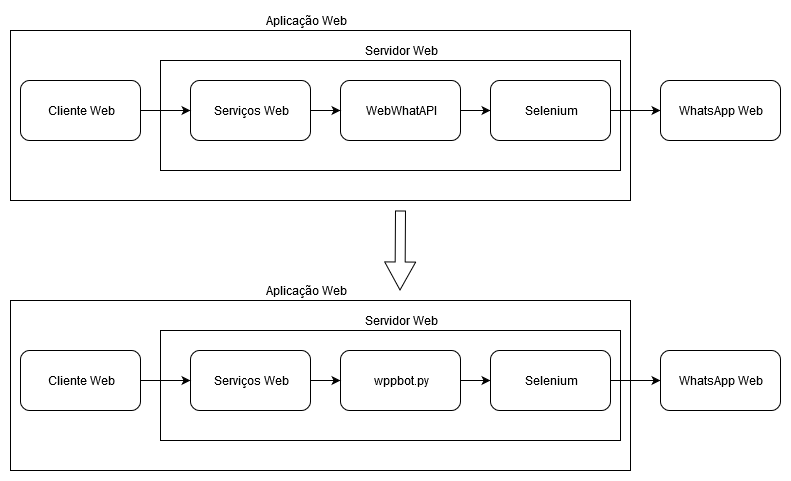
\includegraphics[width=\textwidth]{img/withWebWhatAPI.png}
    \caption{Substituição da ferramenta WebWhatAPI pela ferramenta wppbot.py, a ser criada junto com o presente trabalho}
    \centering
    \label{fig:webWhatAPIChange}
\end{figure}

Para o desenvolvimento da aplicação Web, foi decidido utilizar do \textit{framework} \textit{Flask}\footnote{https://palletsprojects.com/p/flask/}. \textit{Flask} é um \textit{framework} de aplicação web leve e minimalista que utiliza a linguagem Python. O fato da linguagem de desenvolvimento do framework ser a mesma utilizada para o desenvolvimento do Web Scrapper foi um dos principais motivos da escolha do mesmo. O seu minimalismo também foi um fator decisivo para a escolha pois auxilia para que os desenvolvedores possam focar em desenvolver, evitando ter que fazer uma serie de configurações complexas que outros \textit{frameworks} mais robustos e complexos exigem. Como é pretendido que o mesmo possa rodar em serviços de computação em nuvem, sua leveza também se torna um fator importante devido a redução de custos que isso leva.

Para que seja possível a implantação dessa aplicação pelo usuário de uma forma fácil, foi utilizado a ferramenta \textit{Docker}\footnote{https://www.docker.com}. Docker é uma ferramenta que permite que desenvolvedores criem arquivos de configuração que define todas as dependências da aplicação e ao usuário que rode a mesma com apenas um comando. A depender do serviço de computação em nuvem a ser utilizado, basta usar a interface do mesmo para passar qual a \textit{URL} da imagem docker da aplicação que o mesmo fará todo o resto do trabalho. O usuário precisará apenas acessar a \textit{URL} informada para acessar a aplicação. Outra vantagem do uso dessa ferramenta é que ela pode ser configurada em computadores domésticos.



% ### Sobre desenvolvimento
% Abordar tecnologias utilizadas e justificá-las. 
% Qual a stack de desenvolvimento? 
% Python, Selenium, Flask
% Qual a stack de deploy?
% Docker
% Onde é mantido "manual" e formas de contribuição.

% ## Sobre resultados:

% Como é o sistema implementado (com imagens) e o que é possível fazer com ele?

% Exemplo de output do sistema.

% Pequena jornada do usuário desde "baixar" até coletar os dados, seguindo o fluxo principal.

% ## Sobre desenvolvimento

% ### Selenium

% Paragrafo introduzindo necessidade da ferramenta para fazer o Web Scrapper

% O que é o Selenium

% Qual a abordagem que estamos fazendo no uso.

% ### Flask

% Introduzir a necessidade do desenvolvimento do web-service

% O que é o Flask e pq Flask

% Qual a abordagem

% ### Docker

% Introduzir necessidade de criação de container.

% O que é docker (?) e pq

% Qual a abordagem com o docker

% ### Github

% Introduzir necessidade de um local para manter o repositório de forma aberta, onde é possível manter documentação e guia de como mais pessoas contribuírem pra manter e melhor a ferramenta.

% O que é o Github (?) e pq

% Como será mantido a documentação e guia de contribuição.